%%%%%%%%%%%%%%%%%%%%%%%%%%%%%%%%%%%%%%%%%%%%%%%%%%%%%%%%%%%%%%%%%%%%%%
% LaTeX Example: Project Report
%
% Source: http://www.howtotex.com
%
% Feel free to distribute this example, but please keep the referral
% to howtotex.com
% Date: March 2011 
% 
%%%%%%%%%%%%%%%%%%%%%%%%%%%%%%%%%%%%%%%%%%%%%%%%%%%%%%%%%%%%%%%%%%%%%%
% How to use writeLaTeX: 
%
% You edit the source code here on the left, and the preview on the
% right shows you the result within a few seconds.
%
% Bookmark this page and share the URL with your co-authors. They can
% edit at the same time!
%
% You can upload figures, bibliographies, custom classes and
% styles using the files menu.
%
% If you're new to LaTeX, the wikibook is a great place to start:
% http://en.wikibooks.org/wiki/LaTeX
%
%%%%%%%%%%%%%%%%%%%%%%%%%%%%%%%%%%%%%%%%%%%%%%%%%%%%%%%%%%%%%%%%%%%%%%
% Edit the title below to update the display in My Documents
%\title{Project Report}
%
%%% Preamble
\documentclass[paper=a4, fontsize=11pt]{scrartcl}
\usepackage[T1]{fontenc}
\usepackage{fourier}
\usepackage{hyperref}

\hypersetup{
	colorlinks=true,       % false: boxed links; true: colored links
	linkcolor=red,          % color of internal links 
	urlcolor=cyan           % color of external links
}


\usepackage[english]{babel}															% English language/hyphenation
\usepackage[protrusion=true,expansion=true]{microtype}	
\usepackage{amsmath,amsfonts,amsthm} % Math packages
\usepackage[pdftex]{graphicx}	
\usepackage{url}
\usepackage{xcolor}

%%% Custom sectioning
\usepackage{sectsty}
\allsectionsfont{\centering \normalfont\scshape}
\usepackage{tikz}
\usetikzlibrary{chains,shapes.multipart}
\usepackage{pgf}
\usepackage{tikz}
\usetikzlibrary{arrows,automata}

%%% Custom headers/footers (fancyhdr package)
\usepackage{fancyhdr}
\pagestyle{fancyplain}
\fancyhead{}											% No page header
\fancyfoot[L]{}											% Empty 
\fancyfoot[C]{}											% Empty
\fancyfoot[R]{\thepage}									% Pagenumbering
\renewcommand{\headrulewidth}{0pt}			% Remove header underlines
\renewcommand{\footrulewidth}{0pt}				% Remove footer underlines
\setlength{\headheight}{13.6pt}


%%% Equation and float numbering
\numberwithin{equation}{section}		% Equationnumbering: section.eq#
\numberwithin{figure}{section}			% Figurenumbering: section.fig#
\numberwithin{table}{section}				% Tablenumbering: section.tab#


%%% Maketitle metadata
\newcommand{\horrule}[1]{\rule{\linewidth}{#1}} 	% Horizontal rule

\title{
	%\vspace{-1in} 	
	\usefont{OT1}{bch}{b}{n}
	\normalfont \normalsize \textsc{School of random department names} \\ [25pt]
	\horrule{0.5pt} \\[0.4cm]
	\huge Efficient modeling of timeouts in PRISM \\
	\horrule{2pt} \\[0.5cm]
}
\author{
	\normalfont 								\normalsize
	Thomas Mari, M\'{a}rio Uhr\'{i}k\\[-3pt]		\normalsize
	\today
}
\date{}

\usepackage{listings}
\usepackage{color}
\usepackage{float}


%% BEGIN PRISM CODE LISTING 
\definecolor{dkgreen}{rgb}{0,0.6,0}
\definecolor{gray}{rgb}{0.5,0.5,0.5}

\lstset{frame=tb,
	language=Java,
	aboveskip=1mm,
	belowskip=1mm,
	showstringspaces=false,
	columns=flexible,
	basicstyle={\fontsize{8.8}{8.5}\ttfamily},
	numbers=none,
	numberstyle=\tiny\color{gray},
	keywordstyle=\color{blue},
	commentstyle=\color{dkgreen},
	breaklines=true,
	breakatwhitespace=true,
	tabsize=3,
	morekeywords={event, gsmp, dirac, exponential, uniform, weibull, erlang,
		module, init, rewards, endrewards, label, true, endmodule}
}

%%% Begin document
\begin{document}
	\maketitle
	
	\begin{abstract}
		Phase-type fitting remains the only way of modeling non-Markovian distributions within PRISM model checker.
		When analyzing models with phase-type distributions, it is problematic to obtain results of sufficient precision within reasonable time.
		We ran experimental computations and deduced a reasonable way of obtaining precise analysis results for phase-type fitted PRISM CTMCs.
		Lastly, we hint at an entirely different (and arguably better) approach to handling non-Markovian distributions.
	\end{abstract}
	
	\begin{description}
		
		\item[Keywords:] 	PRISM model checker ; CTMC ; deterministic timeout ; phase-type distribution ; modeling ; analysis
		
	\end{description}
	
	%% keywords here, in the form: keyword \sep keyword
	
	%% MSC codes here, in the form: \MSC code \sep code
	%% or \MSC[2008] code \sep code (2000 is the default)
	
	%% main text
	\section{Introduction}
	\label{S:1}
	
	PRISM \cite{KNP11} and Storm \cite{DBLP:journals/corr/DehnertJK017} are popular tools for modeling and analysis of stochastic systems in continuous time. They use efficient algorithms for analysis of continuous time Markov chains (CTMC). This approach suffers from a severe restriction of modeling power --- the time between transitions must be exponentially distributed. This restriction can be remedied by the use of phase-type distributions, which can approximate any general distribution with arbitrary accuracy by only using exponential distributions \cite{Buchholz:2014:IMP:2683922}. However, the use of phase-type distributions drastically increases the number of states within the CTMC.
	
	In this paper, we experimentally evaluate the precision of the result and required computation time of various approaches to analysis of continuous time stochastic models with deterministic transitions (timeouts). The obtained results are then compared against results of our extension of PRISM capable of efficiently analyzing CTMC with non-Markovian alarms (ACTMC).
	
	
	% \subsection{Subsection One}
	
	% Quisque elit ipsum, porttitor et imperdiet in, facilisis ac diam. Nunc facilisis interdum felis eget tincidunt. In condimentum fermentum leo, non consequat leo imperdiet pharetra. Fusce ac massa ipsum, vel convallis diam. Quisque eget turpis felis. Curabitur posuere, risus eu placerat porttitor, magna metus mollis ipsum, eu volutpat nisl erat ac justo. Nullam semper, mi at iaculis viverra, nunc velit iaculis nunc, eu tempor ligula eros in nulla. Aenean dapibus eleifend convallis. Cras ut libero tellus. Integer mollis eros eget risus malesuada fringilla mattis leo facilisis. Etiam interdum turpis eget odio ultricies sed convallis magna accumsan. Morbi in leo a mauris sollicitudin molestie at non nisl.
	
	% \begin{table}[h]
	% \centering
	% \begin{tabular}{l l l}
	% \hline
	% \textbf{Treatments} & \textbf{Response 1} & \textbf{Response 2}\\
	% \hline
	% Treatment 1 & 0.0003262 & 0.562 \\
	% Treatment 2 & 0.0015681 & 0.910 \\
	% Treatment 3 & 0.0009271 & 0.296 \\
	% \hline
	% \end{tabular}
	% \caption{Table caption}
	% \end{table}
	
	% \subsection{Subsection Two}
	
	% Donec eget ligula venenatis est posuere eleifend in sit amet diam. Vestibulum sollicitudin mauris ac augue blandit ultricies. Nulla facilisi. Etiam ut turpis nunc. Praesent leo orci, tincidunt vitae feugiat eu, feugiat a massa. Duis mauris ipsum, tempor vel condimentum nec, suscipit non mi. Fusce quis urna dictum felis posuere sagittis ac sit amet erat. In in ultrices lectus. Nulla vitae ipsum lectus, a gravida erat. Etiam quam nisl, blandit ut porta in, accumsan a nibh. Phasellus sodales euismod dolor sit amet elementum. Phasellus varius placerat erat, nec gravida libero pellentesque id. Fusce nisi ante, euismod nec cursus at, suscipit a enim. Nulla facilisi.
	
	% \begin{figure}[h]
	% \centering\includegraphics[width=0.4\linewidth]{placeholder}
	% \caption{Figure caption}
	% \end{figure}
	
	% Integer risus dui, condimentum et gravida vitae, adipiscing et enim. Aliquam erat volutpat. Pellentesque diam sapien, egestas eget gravida ut, tempor eu nulla. Vestibulum mollis pretium lacus eget venenatis. Fusce gravida nisl quis est molestie eu luctus ipsum pretium. Maecenas non eros lorem, vel adipiscing odio. Etiam dolor risus, mattis in pellentesque id, pellentesque eu nibh. Mauris nec ante at orci ultricies placerat ac non massa. Aenean imperdiet, ante eu sollicitudin vestibulum, dolor felis dapibus arcu, sit amet fermentum urna nibh sit amet mauris. Suspendisse adipiscing mollis dolor quis lobortis.
	
	% \begin{equation}
	% \label{eq:emc}
	% e = mc^2
	% \end{equation}
	
	\section{Experimental evaluation}
	\label{S:2}
	
	\begin{figure}[H]
		\centering
		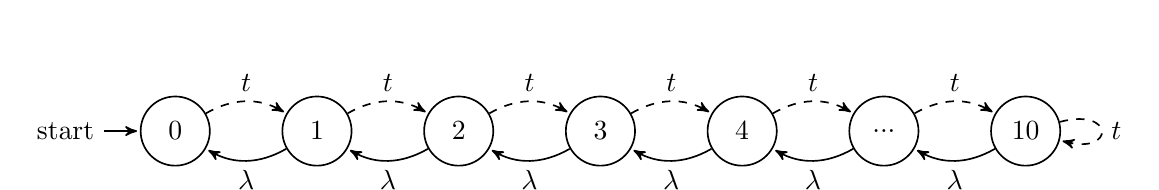
\begin{tikzpicture}[->,>=stealth',shorten >=1pt,auto,node distance=1.8cm,
		semithick]
		\tikzstyle{every state}=[fill=white,draw=black,text=black]
		
		\node[initial,state] (s0)                    {$0$};
		\node[state]         (s1) [right of=s0] {$1$};
		\node[state]         (s2) [right of=s1] {$2$};
		\node[state]         (s3) [right of=s2] {$3$};
		\node[state]         (s4) [right of=s3]       {$4$};
		\node[state]         (sw) [right of=s4,fill=white,text=black]       {...};
		\node[state]         (sn) [right of=sw]       {$10$};
		
		
		
		\path[->, dashed]  
		(s0) edge [bend left]             node {$t$} (s1);
		\path[->]
		(s1) edge [bend left] node {$\lambda$} (s0);
		\path[->, dashed]
		(s1) edge  [bend left]            node {$t$} (s2);
		\path[->]
		(s2) edge [bend left]             node {$\lambda$} (s1);
		\path[->, dashed]
		(s2) edge [bend left]  node {$t$} (s3);
		\path[->]
		(s3) edge [bend left]              node {$\lambda$} (s2);
		\path[->, dashed]
		(s3) edge [bend left]  node {$t$} (s4);
		\path[->]
		(s4) edge [bend left]             node {$\lambda$} (s3);
		\path[->, dashed]
		(s4) edge [bend left]  node {$t$} (sw);
		\path[->]
		(sw) edge [bend left]             node {$\lambda$} (s4);
		\path[->, dashed]
		(sw) edge [bend left]  node {$t$} (sn);
		\path[->]
		(sn) edge [bend left]             node {$\lambda$} (sw);
		\path[->, dashed]
		(sn) edge [loop right]  node {$t$} (sn);
		\end{tikzpicture}
		\caption{Model of a D/M/1/10 queue with production timeout $t = 0.1$ and service rate $\lambda = \frac{ln(2)}{t} \approx 6.931471805599453094$. The deterministic arrival event does not reset when the exponential service event occurs.}
		\label{fig:D/M/1/10}
	\end{figure}
	
	We have chosen to model a D/M/1/10 queue (deterministic arrivals, exponentially distributed service, single server, capacity of 10) as shown in Figure \ref{fig:D/M/1/10}. The deterministic arrivals are approximated by a phase-type distribution, so the model remains a CTMC and can be analyzed by PRISM. The PRISM model we used is shown in Figure \ref{fig:D/M/1/10_PRISM}.
	We computed the steady-state distribution with various values of PRISM termination epsilon $\epsilon$ and the number of phases $k$.
	
	\begin{figure}[H]
		\begin{lstlisting}
		ctmc
		
		const int k;
		const int qCapacity = 10;
		const double timeout = 0.1;
		const double lambda = 6.931471805599453094;
		
		module main
		
		qSize : [0..qCapacity] init 0;
		
		[produce] (qSize <= qCapacity) -> (qSize' = min(qSize+1,qCapacity));
		[consume] (qSize > 0) -> lambda: (qSize' = qSize - 1);
		
		endmodule
		
		module trigger
		
		i : [1..k+1];
		
		[] i < k -> k/timeout : (i'=i+1);
		[produce] i = k -> k/timeout : (i'=1);
		
		endmodule
		\end{lstlisting}
		\caption{PRISM CTMC model of the D/M/1/10 queue as shown in Figure \ref{fig:D/M/1/10} with a phase-type distribution approximating the arrival timeout. The phase-type module \emph{trigger} is used as suggested on the \href{http://www.prismmodelchecker.org/manual/FrequentlyAskedQuestions/PRISMModelling}{PRISM website}. Phase-type parameter $k$ represents the number of phases. Increasing $k$ should improve the approximation of the timeout. }
		\label{fig:D/M/1/10_PRISM}
	\end{figure}
	
	\pagebreak
	\subsection{Obtaining precise results for reference}
	\label{S:2.1}
	
%%%	In order to obtain some steady-state probabilities of reference to compare precision of different tools and engines, we computed the same steady-state probabilities two different ways. The first one is the phase type fitting method described as above (ref to the first page). The second one is by using our PRISM ACTMC implementation with precise termination epsilon.
%%%	 the computation  results are quite similar as shown in picture citation
	 
%%%	 put picture diff_per_stqte 
%%%	 explain picture
	
	%%% little conclusion: we can from now trust the event model as a reference 
	 
	 In order to compare the precision of the results obtained by the experiments, a trustworthy high-precision reference is needed. To achieve this, we used our own PRISM ACTMC implementation, which is capable of analyzing the given model directly without phase-type fitting. Using our implementation, we have computed the steady-state probabilities for very precise termination epsilon $\epsilon = 10^{-20}$ and compared it to the steady-state probabilities obtained by PRISM CTMC with phase-type fitting for $\epsilon = 10^{-16}$ and $k = 800000$. As shown in Figure \ref{fig:diff_storm_dynamic}, the differences between the computations are smaller than $10^6$. Under the hypothesis that the true result is closer to the result obtained from PRISM ACTMC than to the result obtained from Storm, we can conclude that the PRISM ACTMC can serve as reference with precision at least $10^{-6}$.
	 
	 	\begin{figure}[H]
		\begin{center}
			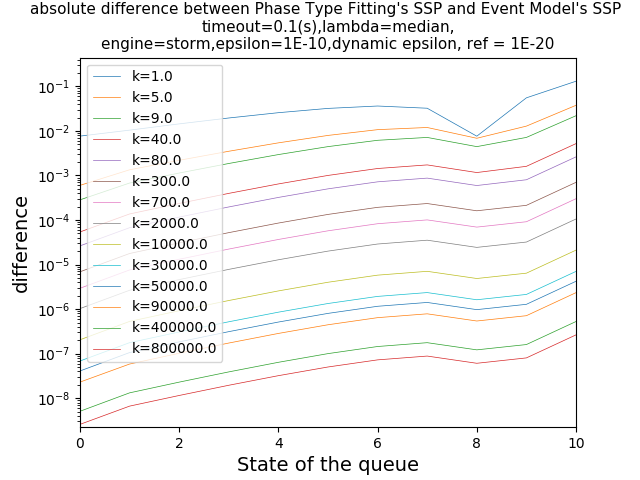
\includegraphics[trim=0.2cm 0cm 0cm 1.35cm,width=15cm, clip]{picture/New_model/1E-10/diff_storm_dynamic.png}
		\end{center}
		\caption{Absolute difference of steady-state probabilities of the CTMC with phase-type fitting ($\epsilon = 10^{-16}$, $k = 800000$) from PRISM ACTMC ($\epsilon = 10^{-20}$).}
		\label{fig:diff_storm_dynamic}
	\end{figure}
	
	\pagebreak
	\subsection{Default absolute termination epsilon $\epsilon = 10^{-6}$}
	\label{S:2.2}
	
	First, we used the PRISM default absolute termination epsilon $\epsilon = 10^{-6}$. The results are shown in Figure \ref{fig:distance_constant_standard_constant_kappa}. For this $\epsilon$, the obtained results are arguably insufficient. Increasing $k$ does little to improve the precision, and only up to about $k \leq 50$, at which point increasing $k$ further starts making the precision worse.
	
	\begin{figure}[H]
		\begin{center}
			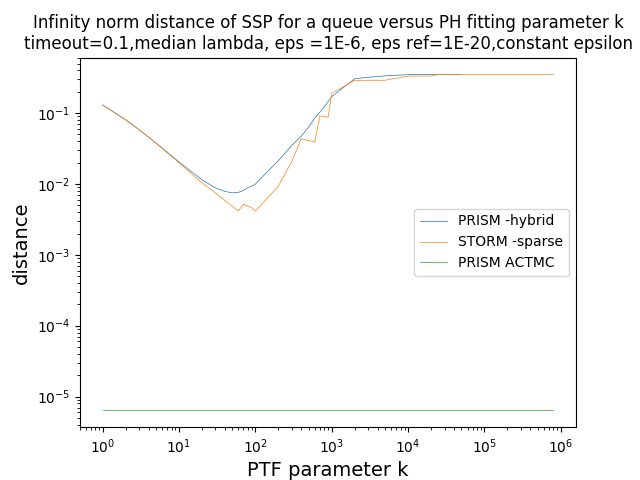
\includegraphics[trim=0.3cm 0cm 0cm 1.35cm,width=15cm, clip]{picture/New_model/1E-6/distance_constant_1E-6.png}
		\end{center}
		\caption{Maximum distance (infinity norm) of the steady-state probabilities from the reference high-precision ACTMC ($10^{-20}$) against various values of $k$ for default absolute termination epsilon $\epsilon = 10^{-6}$. ACTMC results for $\epsilon = 10^{-6}$ are also compared to the reference.}
		\label{fig:distance_constant_standard_constant_kappa}
	\end{figure}
	
	\pagebreak
	\subsection{Lowering absolute termination epsilon to $\epsilon = 10^{-10}$}
	\label{S:2.2}
	
	For much lower $\epsilon = 10^{-10}$, the precision of the result improves. However, for higher $k$ the precision continues to deteriorate like in Section \ref{S:2.2}. The results are shown in Figure \ref{fig:distance_constant_1E-10_constant_kappa}.
	
	
	\begin{figure}[H]
		\begin{center}
			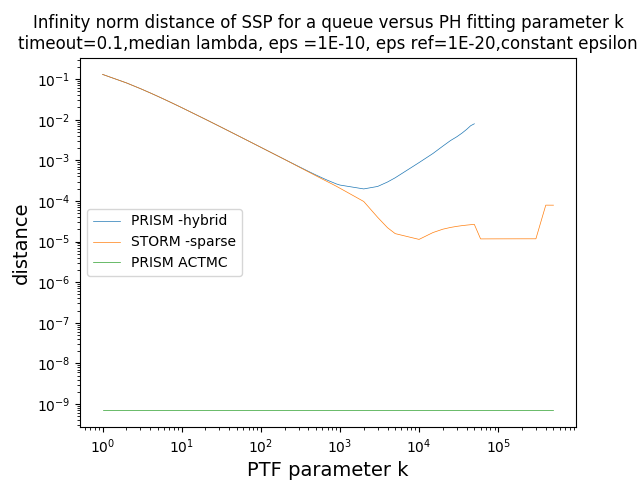
\includegraphics[trim=0.2cm 0cm 0cm 1.35cm,width=15cm, clip]{picture/New_model/1E-10/distance_constant_1E-10.png}
		\end{center}
		\caption{Maximum distance (infinity norm) of the steady-state probabilities from the reference high-precision ACTMC ($10^{-20}$) against various values of $k$ for lowered absolute termination epsilon $\epsilon = 10^{-10}$. ACTMC results for $\epsilon = 10^{-10}$ are also compared to the reference.}
		\label{fig:distance_constant_1E-10_constant_kappa}
	\end{figure}
	
	\pagebreak
	\subsection{Adjusting epsilon $\epsilon = 10^{-10}$ to $k$}
	\label{S:2.3}
	
	Since increasing $k$ increases the amount of phases (intermediate states) and each phase may have error up to $\epsilon$, the actual potential error for each state of the queue is $\epsilon \cdot k$. To compensate for this, we devise a simple formula
	$$\epsilon^{'} = \frac{\epsilon}{k}$$
	where $\epsilon^{'}$ is the adjusted epsilon that should be given to PRISM if precision $\epsilon$ is desired for $k$ phases.
	Using adjusted epsilon, the results get significantly better, as shown in Figure \ref{fig:distance_dynamic_1E-10_constant_kappa}. What's more, the phase-type fitting results now seem to converge towards the reference steadily as $k$ increases. This indicates that this approach is correct, and that the reference is trustworthy.
	
	\begin{figure}[H]
		\begin{center}
			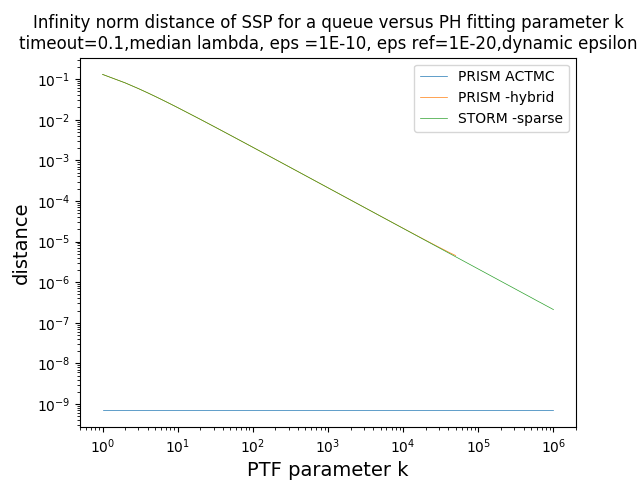
\includegraphics[trim=0.2cm 0cm 0cm 1.35cm,width=15cm, clip]{picture/New_model/1E-10/distance_dynamic_1E-10.png}
		\end{center}
		\caption{Maximum distance (infinity norm) of the steady-state probabilities from the reference high-precision ACTMC ($10^{-20}$) against various values of $k$ for lowered and adjusted absolute termination epsilon $\epsilon = 10^{-10}$. ACTMC results for $\epsilon = 10^{-10}$ are also compared to the reference.}
		\label{fig:distance_dynamic_1E-10_constant_kappa}
	\end{figure}
	
	\subsection{Required computation time to obtain precise results}
	\label{S:2.4}
	
	Although we have shown it is possible to obtain relatively precise results using phase-type distributions, the precision comes at a rather steep cost in computation time. This is shown in Figure \ref{fig:performance_dynamic}. Note that even though Storm is one of the fastest available tools, it still struggles to deliver good precision within reasonable time. The computations all ran on the same virtual machine under same conditions\footnote{Running in a virtual machine might have reduced the performance. The virtual machine we used is available at the \href{http://www.stormchecker.org/documentation/vm/vm.html}{Storm website}.}.
	
	\begin{figure}[H]
		\begin{center}
			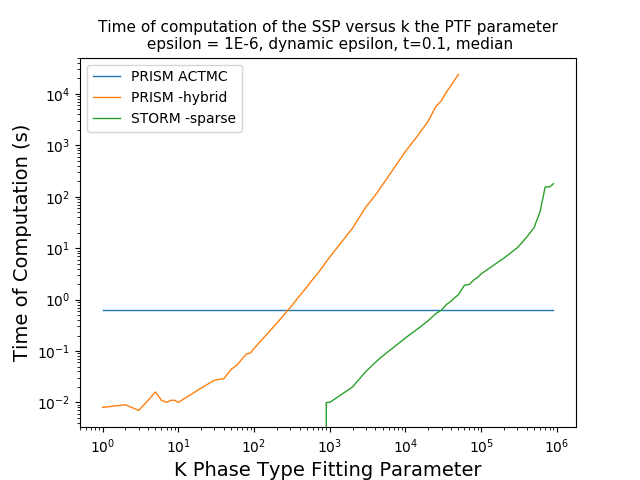
\includegraphics[trim=0.2cm 0cm 0cm 1.35cm,width=15cm, clip]{picture/New_model/1E-6/performance_dynamic.png}
		\end{center}
		\caption{Time of computation in seconds of the steady-state probabilities against various values of $k$ for lowered and adjusted absolute termination epsilon $\epsilon = 10^{-10}$, i.e. corresponding to the data shown in Figure \ref{fig:distance_dynamic_1E-10_constant_kappa}. The computation of our PRISM ACTMC is constant in regards to $k$ because it does not use phase-type fitting. }
		\label{fig:performance_dynamic}
	\end{figure}
	
	\pagebreak
	\section{Conclusion}
	We have presented a reliable method for high-precision analysis of PRISM CTMC models with phase-type distributions, that is, adjusting the termination epsilon by the number of phases. However, the large number of phases drastically increases the computation time.
	
	For better performance, we suggest usage of more specialized tools that can deal with non-Markovian distributions directly, without phase-type fitting. Our PRISM ACTMC extension\footnote{Our PRISM ACTMC extension is not fully completed yet and lacks optimization. It will be officially released later, but early development version is available at \href{https://github.com/VojtechRehak/prism-gsmp}{https://github.com/VojtechRehak/prism-gsmp}.} has delivered results with sufficient precision a lot faster.
	
	
	%% The Appendices part is started with the command \appendix;
	%% appendix sections are then done as normal sections
	%% \appendix
	
	%% \section{}
	%% \label{}
	
	%% References
	%%
	%% Following citation commands can be used in the body text:
	%% Usage of \cite is as follows:
	%%   \cite{key}          ==>>  [#]
	%%   \cite[chap. 2]{key} ==>>  [#, chap. 2]
	%%   \citet{key}         ==>>  Author [#]
	
	%% References with bibTeX database:
	
	\bibliographystyle{model1-num-names}
	\bibliography{sample.bib}
	
	%% Authors are advised to submit their bibtex database files. They are
	%% requested to list a bibtex style file in the manuscript if they do
	%% not want to use model1-num-names.bst.
	
	%% References without bibTeX database:
	
	% \begin{thebibliography}{00}
	
	%% \bibitem must have the following form:
	%%   \bibitem{key}...
	%%
	
	% \bibitem{}
	
	% \end{thebibliography}
	
	
\end{document}\\

